\documentclass[12pt]{ctexart}

%% 页面边距设置
\usepackage{geometry}
\geometry{a4paper, left=3.18cm, right=3.18cm, top=2.54cm, bottom=2.54cm}

%% 页眉和页脚设置
\usepackage{fancyhdr} % 引入 fancyhdr 包: 用于自定义页眉和页脚
\usepackage{lastpage} % 引入 lastpage 包: 用于获取总页数
\pagestyle{fancy}     % 设置页眉和页脚样式为 fancy
\fancyhf{}            % 清空默认的页眉和页脚
\fancyhead[C]{\textbf{标题模板}} % 页眉标题
\fancyfoot[C]{第 \thepage 页,共 \pageref{LastPage} 页}

%% 调整页眉高度
\setlength{\headheight}{14.5pt} % 设置页眉高度为 14.5pt
\addtolength{\topmargin}{-1.5pt} % 调整顶部边距以补偿页眉高度的增加

%% 字体和格式设置
\usepackage{fontspec}
\setmainfont{Times New Roman}  % 英文字体(想使用默认字体请注释)

%% 行间距和段落格式
\usepackage{setspace}
\setstretch{1.5} % 设置行间距为 1.5 倍
\setlength{\parskip}{0.5\baselineskip} % 段后间距为 0.5 行
\setlength{\parindent}{2em} % 首行缩进 2 个字符

%% 使用 ulem 宏包
\usepackage[normalem]{ulem} % 引入 ulem 包: 用于下划线和删除线等文本样式

%% 图片和图形设置
\usepackage{graphicx} % 引入 graphicx 宏包,用于插入图片

%% 表格设置
\usepackage{tabularx} % 引入 tabularx 宏包
\usepackage{booktabs} % 引入 booktabs 宏包,用于表格线条美化
\usepackage{array} % 引入 array 宏包,用于表格列格式设置
\usepackage{makecell} % 引入 makecell 包: 用于表格单元格内换行

%% 列表样式设置
\usepackage{enumitem} % 引入 enumitem 包: 用于自定义列表样式
% 比如:
% \begin{enumerate}[label=\roman*]  % 使用罗马数字编号,不使用默认的阿拉伯数字
% \end{enumerate}

%% 参考文献格式包
\usepackage[sort]{gbt7714} % 引入 gbt7714 包: 用于参考文献格式


\begin{document}

% \nocite{*} % 引用所有参考文献(如果你需要将reference.bib中的所有文献都列出,请使用;如果只需要列出在正文引用的文献,请注释掉这一行)

%% 评分表(若不需要请注释掉)
\pagenumbering{gobble} % 评分表页不显示页码
\begin{titlepage}
    { % 使用内部块
        \centering % 整个页面居中    
        {\bfseries\Large 深圳大学研究生课程期末论文评分表 \\[0.8cm]}
        \raggedright                % 段落从左对齐,避免段落居中影响正文

        \zihao{-4} % 设置正文字体为小四号

        \noindent
        课程名称:\underline{\hspace{4cm}课程的名称\hspace{4.4cm}}

        \noindent
        论文题目:\underline{\hspace{1cm}请输入论文标题(通过hspace控制横线长度)\hspace{1cm}}

        \noindent
        学\hspace{2em}号:\underline{\hspace{1cm}0123456789\hspace{1cm}} \hspace{1em} 姓\hspace{2em}名:\underline{\hspace{3em}名字\hspace{3em}}

        \vspace{0.5cm} % 表格下方留出 0.5cm 的空白

        \raggedright                % 段落从左对齐,避免段落居中影响正文
        \setstretch{1.25}            % 设置下面段落行间距为 1.25 倍
        \setlength{\parskip}{0pt}   % 段后间距设为 0
        % \renewcommand{\arraystretch}{1.8} % 行距增大,视觉美观
        % \setlength{\tabcolsep}{3pt}       % 列间距调整
        % 使用 tabularx 表格
        % 表格部分
        \renewcommand{\arraystretch}{1.7}   % 行距增大,视觉美观
        \begin{tabularx}{\textwidth}{|>{\centering\arraybackslash}m{5em}|X|>{\centering\arraybackslash}m{4em}|>{\centering\arraybackslash}m{4em}|}
            \hline  % 划线
            \textbf{指标} & \textbf{评分标准} & \textbf{分值} & \textbf{得分} \\
            \hline
            文献 & 文献资料是否恰当、详实;是否具有代表性;是否有述有评。 & 10 &  \\
            \hline
            选题 & 选题是否新颖;是否有理论意义或实用价值;是否与授课内容相符。 & 10 &  \\
            \hline
            规范 & 篇幅字数在规定要求范围内;文字表达是否准确、流畅;论述是否具有论辩性;图表计量单位是否规范;是否符合学术道德规范,论文独立完成,无抄袭现象。 & 30 &  \\
            \hline
            论证 & 研究方案是否具有可行性;是否能较好运用所学知识,观点明确;思路是否清晰;逻辑是否严密;结构是否严谨;论证是否充分。 & 30 &  \\
            \hline
            实用价值 & 调研成果是否具有实际应用价值;是否提出了可行的建议或解决方案;是否对相关领域有参考意义;是否体现创新思维。 & 20 &  \\
            \hline
            其他意见(选填) & \multicolumn{3}{l|}{} \\ % 不使用'\rule{10cm}{0pt}',这样以防表格最右端的线不贴合表格,出现短断裂(如下一行所示,可以取消下一行的注释对比效果)
            % 其他意见(选填) & \multicolumn{3}{l|}{\rule{10cm}{0pt}} \\
            \hline
            \multicolumn{2}{|l|}{\textbf{任课教师签名:}\rule{7cm}{0pt}} & \multicolumn{2}{l|}{\textbf{总分:}} \\  % 不使用'\rule{3cm}{0pt}',这样以防表格最右端的线不贴合表格,出现短断裂(如下一行所示,可以取消下一行的注释对比效果)
            % \multicolumn{2}{|l|}{任课教师签名:\rule{7cm}{0pt}} & \multicolumn{2}{l|}{总分:\rule{3cm}{0pt}} \\
            % \hline  % 不使用\hline实线,使两行在PDF中紧密相连,从视觉上变成一行
            \multicolumn{2}{|l|}{\hspace{13em}年\underline{\hspace{1cm}}月\underline{\hspace{1cm}}日} & \multicolumn{2}{l|}{}\\
            \hline
        \end{tabularx}

        \vspace{0.5cm} % 表格下方留出 0.5cm 的空白
        \small
        \noindent
        1. 该表应在期末考试前由任课教师发给学生,告知学生论文评分标准;\\
        2. 学生应在提交期末论文时,封面附上该表并补充填写好表格基本个人信息。
    }
\end{titlepage} % 加载评分表
\newpage                % 换页

%% 诚信承诺书(若不需要请注释掉)
\pagenumbering{gobble} % 诚信承诺书页不显示页码
% 学术诚信承诺书页
\begin{titlepage}
    { % 使用内部块
        \centering % 整个页面居中

        {\bfseries \Large 深圳大学研究生课程论文学术诚信承诺书 \\[1.5cm]}
        \raggedright                % 段落从左对齐,避免段落居中影响正文
        \setstretch{1.8}            % 设置下面段落行间距为 1.8 倍
        \setlength{\parskip}{0pt}   % 段后间距设为 0
        \setlength{\parindent}{2em} % 首行缩进 2 个字符

        \zihao{4} % 设置正文字体为四号
        
        本人在此声明所提交的课程论文 \underline{\hspace{6em}}(论文标题)是本人独立完成的,具有原创性,并且未抄袭、剽窃他人成果或侵犯他人的知识产权。本声明书详细阐述以下内容:

        1. 本人郑重声明,课程论文的所有内容和观点均源自本人的研究和分析,未从其他来源直接复制或翻译。

        2. 对于其他作者或研究人员的观点、数据、图片、图表等引用和参考,本人已按照学校规定的引用标准进行准确的引用和注明,并在文中明确标明了引用部分。

        3. 本人保证,课程论文中使用的所有文献、资料和其他来源均已在参考文献部分列出,且准确无误地注明了相关信息,包括作者、出版年份、出版社或期刊名称等。

        4. 本人明确知晓学术不端行为的严重性,包括但不限于抄袭、剽窃、造假、篡改数据等。本人承诺,在课程论文的整个研究和撰写过程中,坚守学术道德原则,维护学术诚信。

        我郑重承诺以上内容的真实性,并愿意为我所提交的课程论文的原创性负全部责任。

        \vspace{1cm}
        % \zihao{-4} % 设置签名部分字体为小四号
        \setlength{\parindent}{0pt} % 下一行段首不缩进
        
        %%  下面的签名行可以使用图片或手写签名
        % 下面的图片需要你自己准备,放在 Imgs 文件夹下,并命名为 Electronic-Signature.jpg
        % 论文作者签名:\raisebox{-0.5\height}{\includegraphics[width=4cm]{Imgs/Electronic-Signature.jpg}} \hfill 日期:\underline{\hspace{0.3cm}2025\hspace{0.3cm}}年\underline{\hspace{0.3cm}06\hspace{0.3cm}}月\underline{\hspace{0.3cm}12\hspace{0.3cm}}日 % \raisebox{-0.5\height}{...} 表示把图片整体往上提半个图片高度,从而大致与前面的文本基线对齐;这样文字与图片看起来是在一条水平线上;这一种做法在签名行、行内小图标等场景非常常用
        
        % 如果需要手写签名,可以使用 \underline{\hspace{4cm}} 代替图片
        论文作者签名:\underline{\hspace{8em}} \hfill 日期:\underline{\hspace{0.3cm}2025\hspace{0.3cm}}年\underline{\hspace{0.3cm}06\hspace{0.3cm}}月\underline{\hspace{0.3cm}12\hspace{0.3cm}}日
    }
\end{titlepage}

%% LaTeX 字体命令参考字体
% LaTeX 实际字号会依赖于 documentclass 里设定的基本字号(比如 10pt、11pt、12pt)
% 下面我以常用的 12pt 版式为例给你做标准对照,符合国内论文排版习惯,方便在论文中选用:
% LaTeX 命令     大致字号     中文习惯称呼     常用场景
% \Huge         24pt        小初(接近)     论文封面、论文题目
% \huge         20pt        小一(接近)     正文一级大标题
% \LARGE       17pt        二号(接近)     封面副标题、扉页标题
% \Large       14pt        三号(接近)     正文大标题、小节标题
% \large       12pt        小四(正文字号) 正文内适当放大
% \normalsize  12pt        小四             正文默认
% \small       11pt        五号偏小         脚注、附表说明
% \footnotesize 10pt        五号             脚注、参考文献
% \scriptsize  8pt         小五             表格中小字、附注
% \tiny        6pt         小六             非常小,几乎不用


%% 补充国内常用 \zihao{} 对照(学位论文最常用)
%| \zihao{0} | 42pt | 初号 |
%| \zihao{-0} | 36pt | 小初号 |
%| \zihao{1} | 26pt | 一号 |
%| \zihao{2} | 22pt | 二号 |
%| \zihao{3} | 16pt | 三号 |
%| \zihao{4} | 14pt | 四号(正文字号推荐) |
%| \zihao{5} | 10.5pt | 五号 | % 加载学术诚信承诺书
\newpage                % 换页

%% 课程论文封面(若不需要请注释掉)
\pagenumbering{gobble} % 课程论文封面页不显示页码
\begin{titlepage}
    \centering

    \vspace*{\fill} % 垂直居中(在页面顶部插入一段“可拉伸的垂直空白”,让内容自动垂直居中)
    \begin{center}
        {\Huge \textbf{深圳大学研究生课程论文}} \\[1cm]
    \end{center}
    
    \zihao{4}
    \setlength{\tabcolsep}{0.8em}     % 设置表格列间距为 0.8 em
    \renewcommand{\arraystretch}{2} % 设置表格行距为 2 倍
    
    \begin{center}
        \begin{tabular}{p{15em}p{12em}}
            %% 如果题目单行放得下,请直接使用 \underline{\hspace{9.5em}} 包裹题目内容
            题目 \underline{\hspace{3.5em}论文的题目\hspace{3.5em}} & 成绩\makecell[l]{\\ \underline{\hspace{9.5em}}} \\
            %% 如果题目双行才放得下,请使用 \makecell[l]{{...}} 包裹题目内容
            % 题目 \makecell[l]{{\hspace{1em}基于区块链的联邦学习\hspace{1em}} \\ \underline{\hspace{0.5em}数据共享机制设计与优化\hspace{0.5em}}} & 成绩\makecell[l]{\\ \underline{\hspace{9.5em}}} \\
            专业\underline{\hspace{3.5em}计算机技术\hspace{3.5em}} & \makecell[l]{{课程名称{\hspace{1em}课程名称\hspace{1em}}}\\{代\hspace{2em}码\underline{\hspace{2em}11234567\hspace{2em}}}} \\
            年级\underline{\hspace{4.5em}20xx级\hspace{4.5em}} & 姓名\underline{\hspace{3em}姓 名\hspace{3.5em}} \\
            学号\underline{\hspace{3.5em}0123456789\hspace{3.5em}} & 时间\underline{\hspace{1em}2025\hspace{1em}}年\underline{\hspace{1em}06\hspace{1em}}月 \\
            任课教师\underline{\hspace{2.5em}教师的名字\hspace{2.5em}} & \\

            %% 如果需要添加更多行,可以继续在这里添加

            %% 注意,你可以通过控制表格的列宽和行高来调整内容的排版效果,或者\hspace{1em}等命令来调整空白宽度
        \end{tabular}
    \end{center}

    \vspace*{\fill} % 垂直居中(在页面底部也插入一段“可拉伸空白”,与顶部那段 `\vspace*{\fill}` 相配合,保证标题页内容整体垂直居中对称)
\end{titlepage} % 加载课程论文封面
\newpage                % 换页  

%% 封面页设置(若不需要请注释掉)
% \title{基于区块链的联邦学习数据共享机制设计与优化}
% \author{吴勇进}
% \date{\today}
% \maketitle
% \thispagestyle{fancy} % 强制第一页使用 fancy 页眉和页脚,否则第一页默认使用 plain 样式,导致第一页无法显示前面定义的页眉和页脚设置;如果需要封面页与正文的页眉页脚不一致请注释掉这一行

%% 独立标题页
\begin{titlepage} % 开启一个单独的标题页环境。它会自动插入分页,并允许在这个页面上自由排版,适合封面、标题等单页内容·
    \centering    % 居中对齐
    \vspace*{\fill} % 在页面顶部添加垂直空间,使内容垂直居中
    {\bfseries\Huge 标题模板 \\[1cm]}   % 粗体、居中、标题(按顺序分别是:`{ ... }`:局部作用域,控制这行内部的字体格式,不影响后续;`\bfseries`:粗体字,即Bold;`\Huge`:字号非常大,适合标题,比 `\huge` 还大一级);论文标题;`\\[1cm]`:换行,并在这一行后额外插入 1cm 的垂直空白,让标题和作者名之间留出适当间距)
    {\Large 课程名称:XXX \\[0.5cm]} % 课程名称
    {\Large 课程代码:XXXXXX \\[0.5cm]} % 课程代码
    {\Large 指导教师(授课老师):XXX \\[0.5cm]} % 指导教师
    {\Large 学院:XXX \\[0.5cm]} % 学院名称
    {\Large 专业:XXX \\[0.5cm]} % 专业名称
    {\Large 姓名:XXX \\[0.5cm]} % 姓名
    {\Large 学号:XXXXXXXX \\[0.5cm]} % 学号
    {\Large 完成日期:\today \\[0.5cm]} % 完成日期
    {\Large 提交日期:XXXX年XX月XX日 \\[0.5cm]} % 提交日期
    \vspace*{\fill} % 在页面底部添加垂直空间,使内容垂直居中
\end{titlepage}

%% 摘要页设置
\pagenumbering{Roman}   % 设置摘要页的页码格式为罗马数字(Roman为大写、roman为小写)
\pagestyle{plain}       % 使用 plain 样式,清空页眉,仅显示页脚页码
\section*{摘要} % 摘要不需要编号
\addcontentsline{toc}{section}{摘要} % 手动将摘要添加到目录

在此处填写您的摘要内容

示例:本文围绕XXX展开分析,提出了XXX模型,并探讨了其优势与适用场景。

【关键词】请填写您的关键词,例如:区块链;联邦学习;数据共享;隐私保护;智能合约

\newpage % 换页
\section*{Abstract} 

在此处填写您的英文摘要内容

示例:This paper systematically analyzes XXX and proposes XXX models. The advantages and challenges are discussed in detail.

【Keywords】请填写您的英文关键词,例如:Blockchain; Federated Learning; Data Sharing; Privacy Protection; Smart Contracts % 加载摘要
\newpage                % 换页

%% 目录设置
\pagenumbering{arabic}  % 重新编号为阿拉伯数字
\pagestyle{plain}       % 使用 plain 样式
\tableofcontents        % 生成目录
\newpage                % 换页

\zihao{-4}  % 从正文开始设置字体为小四

%% 加载独立的正文内容文件
\setcounter{page}{1}    % 从正文开始重新编号页码
\pagestyle{fancy}       % 使用 fancy 样式(符合前面对正文页脚设置格式)
\section{引言}
\subsection{背景介绍}
在此处填写背景介绍内容

示例:在大数据和人工智能快速发展的背景下,数据孤岛和隐私保护之间的矛盾日益凸显
\cite{mcmahan2017communication}。联邦学习的提出为这一困境提供了新的思路……

\subsection{报告的目的与重要性}

在此处填写报告的目的与重要性内容
% 示例:本报告旨在阐释与梳理区块链技术与联邦学习的深度融合机理,聚焦于二者结合下的数据共享机制设计与优化路径……  % 加载引言
\newpage                % 换页
\section{章节标题示例:技术概述}

\subsection{技术定义与特性}

% 请在此处填写您研究的技术定义与其主要特性说明。
% 示例:
% 本节应简要介绍所研究技术的基本概念、定义、原理以及主要特点,适合引用权威文献支持。

\begin{figure}[htbp]
    \centering
    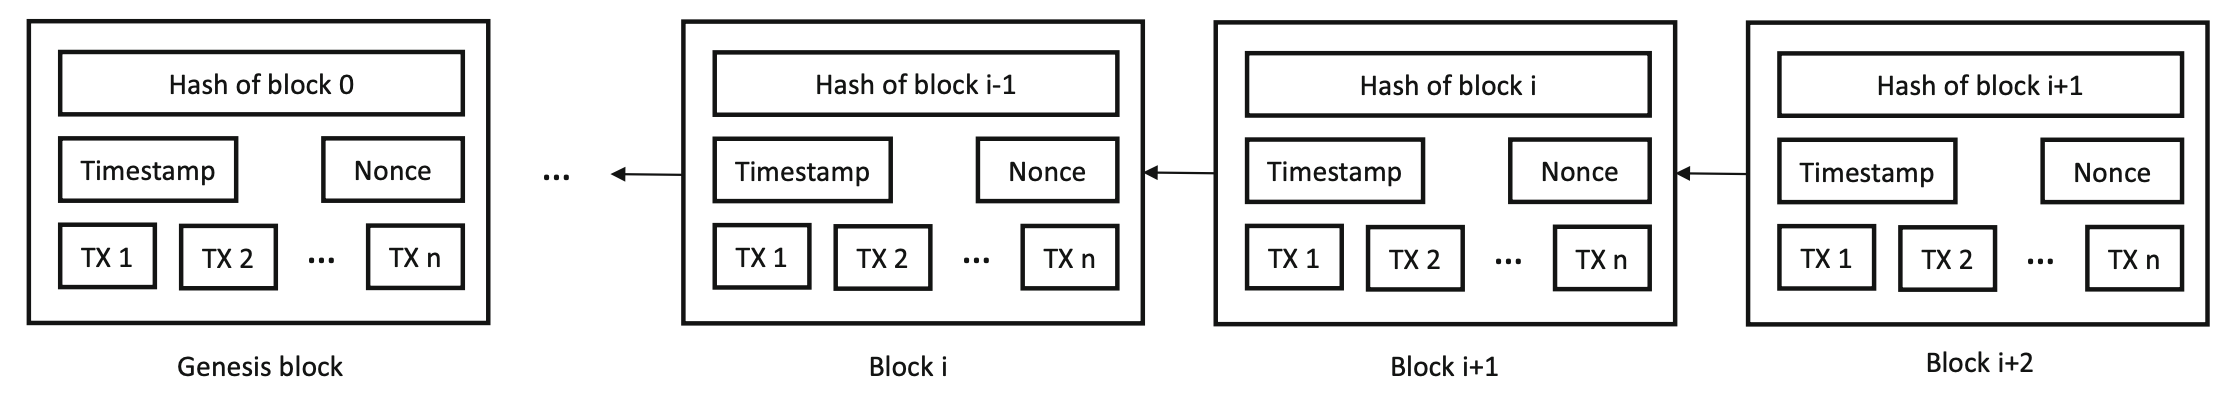
\includegraphics[width=\textwidth]{Imgs/BlockChain.png}
    \caption{示意图示例:此处填写图片说明文字}
    \label{fig:example_structure}
\end{figure}

% 插图说明:
% 使用 \includegraphics 插入图片,推荐图片存放在项目文件夹中的 Imgs 目录下。
% 使用 \caption{} 添加图标题,使用 \label{} 方便文中引用。

\subsection{工作原理}

% 请在此处描述所研究技术的基本工作机制或整体流程。
% 可以使用如下格式描述流程:
% (1)步骤一描述……
% (2)步骤二描述……
% (3)步骤三描述……

% 示例无序列表:
\begin{itemize}
    \item 特性一:请填写特性描述。
    \item 特性二:请填写特性描述。
    \item 特性三:请填写特性描述。
\end{itemize}

% 插入参考文献示例:
% 文中引用示例:\cite{sample2024}
% 请在参考文献文件 reference.bib 中添加相关条目。       % 加载正文内容
\newpage
\section{联邦学习}

\subsection{联邦学习基本概念}
联邦学习(Federated Learning, FL)是一种分布式机器学习框架,在保障数据隐私的前提下,实现多方协同训练机器学习模型\cite{yang2019federated}。与传统集中式训练不同,联邦学习不要求上传原始数据到中央服务器,而是各参与方(客户端)在本地使用自身数据训练模型,仅上传模型更新(如参数梯度)至中央服务器进行聚合,从而形成全局模型,如图\ref{fig:federated_learning_workflow}所示。

\begin{figure}[htbp]
    \centering
    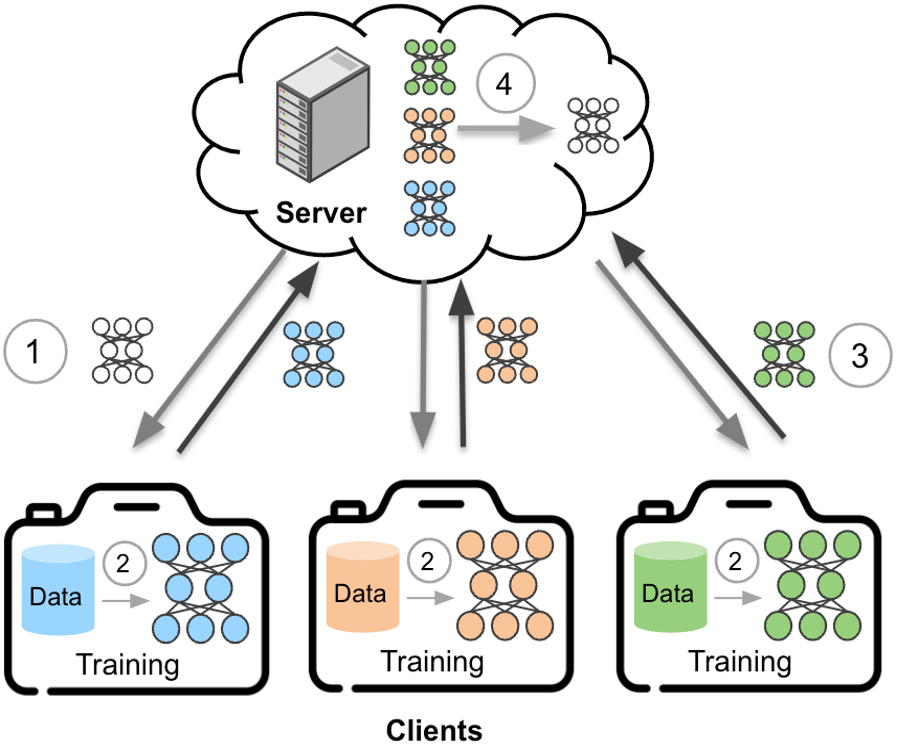
\includegraphics[width=0.6\textwidth]{Imgs/FL-structure.png}
    \caption{联邦学习工作流程总览图}
    \label{fig:federated_learning_workflow}
\end{figure}

该概念最早由Google于2016年提出\cite{mcmahan2017communication},其核心优势在于数据始终保留本地,避免了隐私泄露风险与法律合规问题,同时通过整合多方知识提升模型泛化性能。联邦学习已在医疗、金融、移动终端等数据敏感场景获得广泛应用\cite{zhang2024fedtgp, hard2018federated}。

\subsection{联邦学习的工作流程}
联邦学习的典型流程如图\ref{fig:fl_protocol_round}所示,主要包括以下步骤:

\begin{figure}[htbp]
    \centering
    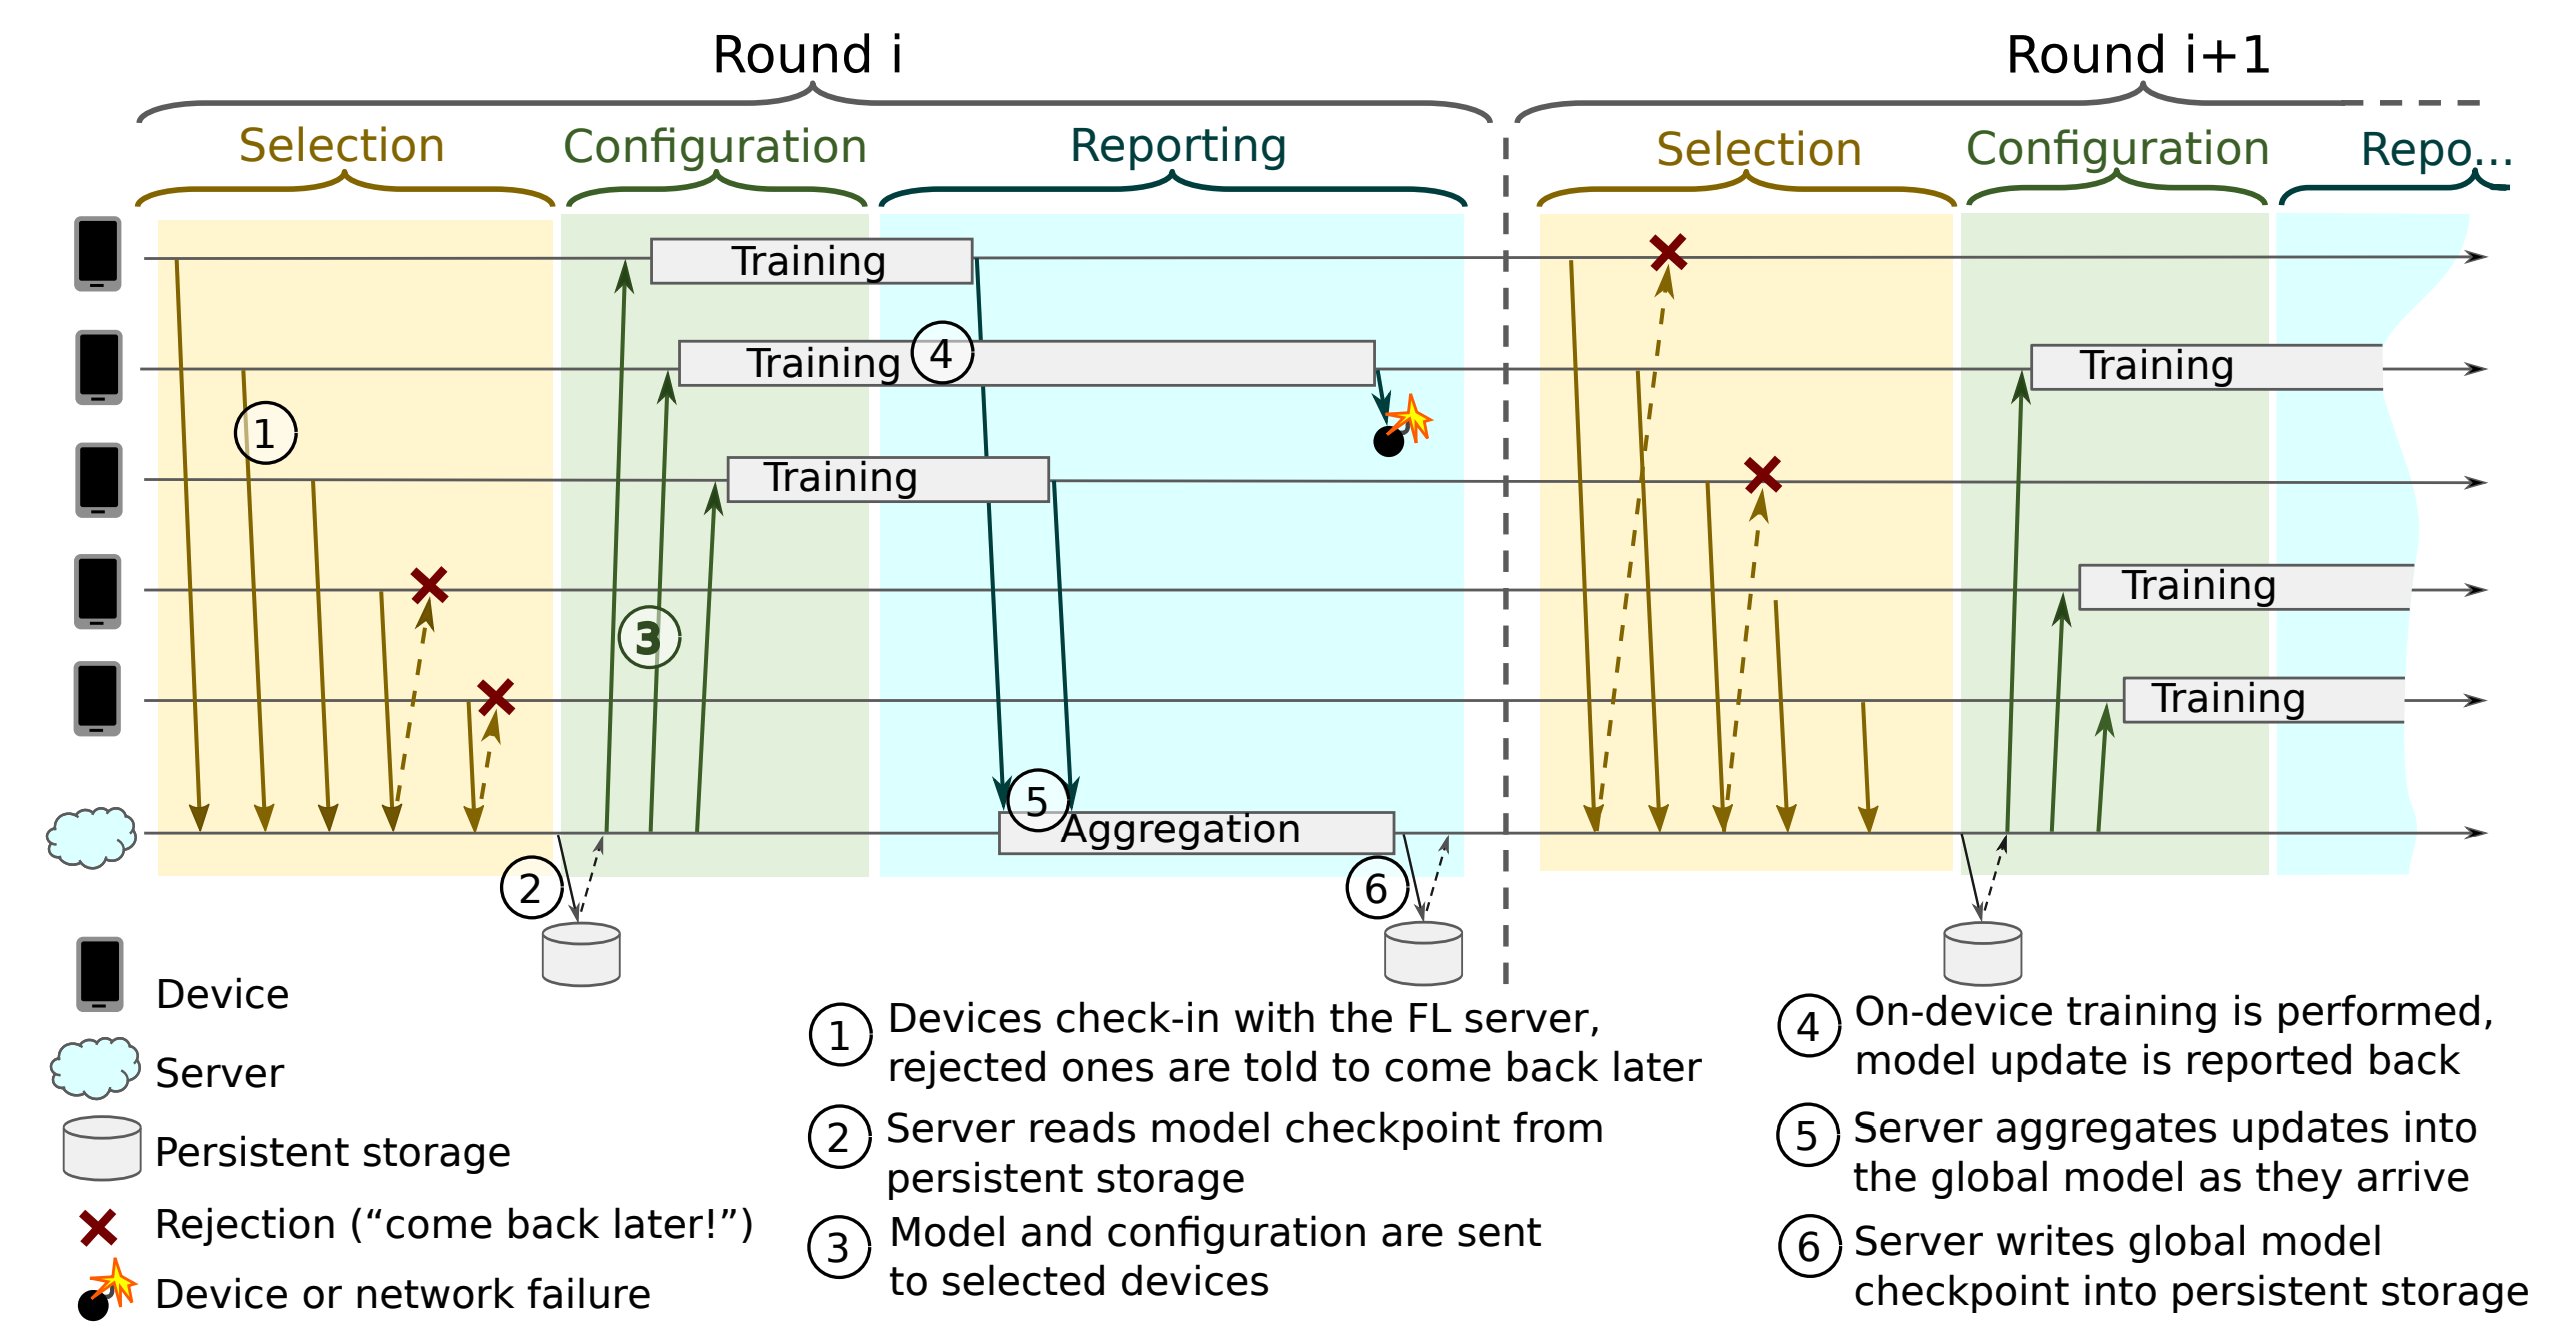
\includegraphics[width=\textwidth]{Imgs/FL-Learning-Protocol.png}
    \caption{典型联邦学习协议轮次流程示意图\cite{bonawitz2019towards}}
    \label{fig:fl_protocol_round}
\end{figure}

\textbf{(1)全局模型初始化与下发:} 服务器初始化全局模型并下发至客户端。\\
\textbf{(2)客户端本地训练:} 客户端在本地数据上训练,更新模型参数。\\
\textbf{(3)本地模型更新上传:} 客户端将加密后的模型更新上传至服务器。\\
\textbf{(4)全局模型聚合:} 服务器采用如FederatedAveraging等算法聚合客户端更新。\\
\textbf{(5)循环迭代直至收敛:} 重复上述过程直至模型收敛或达到设定轮次。

在整个过程中,原始数据从不离开本地,跨节点仅传递模型更新,可结合差分隐私、安全多方计算等技术进一步增强安全性与信任度。

\subsection{联邦学习的主要挑战}
尽管联邦学习在隐私保护方面具备优势,其分布式架构也带来了以下关键挑战\cite{zhu2023blockchain,li2020federated}:

\begin{itemize}
    \item \textbf{信任与安全挑战:} 依赖中心服务器存在单点故障与中毒攻击等安全隐患,需引入稳健聚合、差分隐私等机制提升安全性。
    \item \textbf{缺乏激励机制:} 缺乏合理激励可能导致参与方积极性不足或出现搭便车行为,影响整体训练质量。
    \item \textbf{统计异构性:} 各客户端数据分布差异显著(Non-IID问题),加剧模型收敛困难,影响全局模型泛化性。
    \item \textbf{系统异构性:} 设备性能与网络环境差异大,易产生“慢节点”问题,需设计容错与调度机制适应异构环境。
    \item \textbf{通信负担:} 多轮模型交换带来高通信开销与潜在窃听风险,需借助加密与通信压缩技术优化效率与安全。
    \item \textbf{法规约束:} 需遵循各国数据隐私法规(如GDPR)限制,设计合规的跨境协作方案\cite{li2019impact}。
\end{itemize}

综上,联邦学习在打破数据孤岛方面展现潜力,但仍需解决信任、激励与异构性等技术难题。为应对这些挑战,区块链的去中心化与可编程机制为联邦学习提供了重要补充。下一节将系统探讨区块链赋能下的数据共享机制设计。    % 加载结论
\newpage

%% 引用参考文献
\bibliographystyle{gbt7714-numerical}
\bibliography{reference}

\end{document}

%% LaTeX 字体命令参考字体
% LaTeX 实际字号会依赖于 documentclass 里设定的基本字号(比如 10pt、11pt、12pt)
% 下面我以常用的 12pt 版式为例给你做标准对照,符合国内论文排版习惯,方便在论文中选用:
% LaTeX 命令     大致字号     中文习惯称呼     常用场景
% \Huge         24pt        小初(接近)     论文封面、论文题目
% \huge         20pt        小一(接近)     正文一级大标题
% \LARGE       17pt        二号(接近)     封面副标题、扉页标题
% \Large       14pt        三号(接近)     正文大标题、小节标题
% \large       12pt        小四(正文字号) 正文内适当放大
% \normalsize  12pt        小四             正文默认
% \small       11pt        五号偏小         脚注、附表说明
% \footnotesize 10pt        五号             脚注、参考文献
% \scriptsize  8pt         小五             表格中小字、附注
% \tiny        6pt         小六             非常小,几乎不用


%% 补充国内常用 \zihao{} 对照(学位论文最常用)
%| \zihao{0} | 42pt | 初号 |
%| \zihao{-0} | 36pt | 小初号 |
%| \zihao{1} | 26pt | 一号 |
%| \zihao{2} | 22pt | 二号 |
%| \zihao{3} | 16pt | 三号 |
%| \zihao{4} | 14pt | 四号(正文字号推荐) |
%| \zihao{5} | 10.5pt | 五号 |